\documentclass[twoside,a4paper]{article}
\usepackage{geometry}
\geometry{margin=1.5cm, vmargin={0pt,1cm}}
\setlength{\topmargin}{-1cm}
\setlength{\paperheight}{29.7cm}
\setlength{\textheight}{25.3cm}

% useful packages.
\usepackage{amsfonts}
\usepackage{amsmath}
\usepackage{amssymb}
\usepackage{amsthm}
\usepackage{enumerate}
\usepackage{graphicx}
\usepackage{multicol}
\usepackage{fancyhdr}
\usepackage{layout}
\usepackage{tabularx}
\usepackage{xeCJK}

% some common command
\newcommand{\dif}{\mathrm{d}}
\newcommand{\avg}[1]{\left\langle #1 \right\rangle}
\newcommand{\difFrac}[2]{\frac{\dif #1}{\dif #2}}
\newcommand{\pdfFrac}[2]{\frac{\partial #1}{\partial #2}}
\newcommand{\OFL}{\mathrm{OFL}}
\newcommand{\UFL}{\mathrm{UFL}}
\newcommand{\fl}{\mathrm{fl}}
\newcommand{\op}{\odot}
\newcommand{\Eabs}{E_{\mathrm{abs}}}
\newcommand{\Erel}{E_{\mathrm{rel}}}

\begin{document}

\pagestyle{fancy}
\fancyhead{}
\lhead{俞璐 (3180104284)}
\chead{Project1}
\rhead{2021/04/23}



\section*{I.主程序和测试程序的使用说明}
\hspace{0.8em}
主程序由./main\_test下的main\_1.cpp和main\_2.cpp构成,分别用于两个初值三体问题的数值解的图像的matlab程序的生成。

main\_1.cpp用于第一个初值问题,其输入文件"main1\_input.txt"提供三个值,分别表示所使用的求解方法、
该方法的精度和总步数,例如"Adams\_Bashforth 4 24000"表示希望使用总步数为24000的4阶Adams Bashforth方法求解
第一个初值问题,运行main\_1后得到名为main1\_output.m的matlab脚本文件,在matlab下运行该脚本文件可以得到数值解的
图像。

main\_2.cpp解决的是第二个初值问题,其输入文件为"main2\_input.txt",输入格式同main\_1.cpp,输出文件为"main2\_output.m"。

测试程序由./main\_test下的Test\_1.cpp和Test\_2.cpp构成,它们分别对两个初值问题进行相对应的测试。

Test\_1.cpp用于对第一个初值问题的测试,其输入文件"Test1\_input.txt"提供四个值,分别表示所测试的方法、方法的精度、初始步数、
提升步数的次数。例如"Adams\_Bashforth 4 24000 4",表示测试四阶Adams Bashforth方法在不同步数下的
表现情况,其中初始步数为24000,之后每轮步数乘2,总共提升4轮。对于每一步数,计算相应的误差、CPU计算时间和收敛速度,
结果显示在"Test1.out"文件下。

Test\_2.cpp用于对第二个初值问题的测试,其输入文件为"Test2\_input.txt",其四个输入参数意义同"Test1\_input.txt"四个参数,
输出结果显示在"Test2.out"文件下。

\section*{II.代码的UML图}
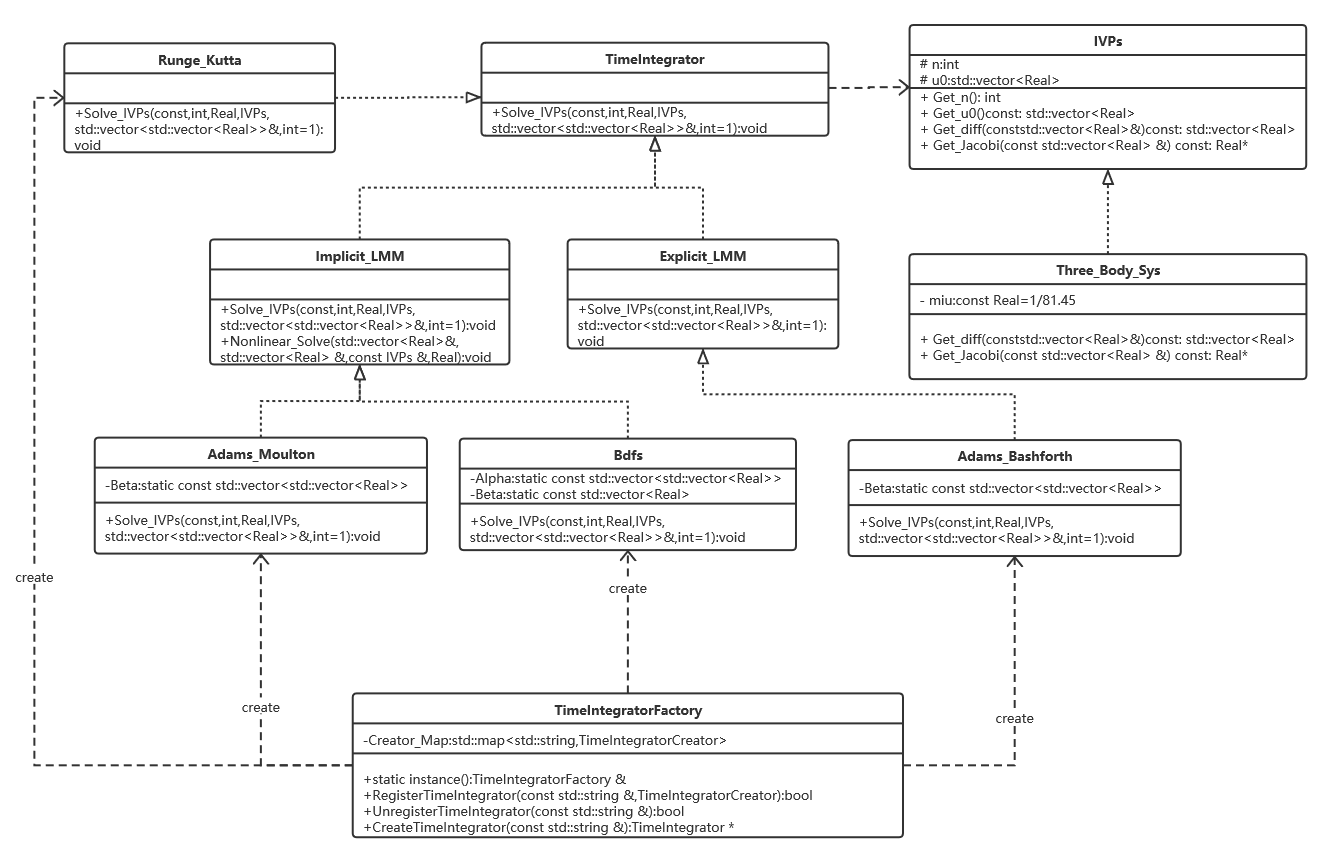
\includegraphics[scale=0.37]{../png/uml.png}

\newpage
\section*{III.步数递增下,不同精度不同方法的误差、CPU时间和收敛速度的计算结果}
\subsection*{III-a. 第一个初值问题}
\hspace{0.8em}
第一个初值问题因为是以$T_1$为周期的,所以可以将初始值$u(0)$视为$u$在$T_1$的精确解,既$u(T_1)=u(0)$。假设一个$p$阶精度的方法在步长为$h$所得到的
数值解$U$在$T_1$的取值为$U^{T_1/h}$,则可以定义误差$E(h)=||U^{T_1/h}-u(T_1)||_{\infty}$。此时由之前所学的收敛性理论可知,若$h$足够的小,我们有
\begin{align}
    E(h)              & =Ch^p+o(h^p),\ \ \  h \rightarrow 0 \\
    \Rightarrow  E(h) & \approx Ch^p
\end{align}
加密网格,使得步长$h$缩小为$\frac{1}{2}h$,此时同样有
\begin{align}
    E(h/2) \approx C(h/2)^p
\end{align}
结合$(2)$可得
\begin{align}
    p\approx \log_2(E(h)/E(h/2))
\end{align}
所以根据$(4)$,我们可以通过前后两次的误差计算收敛速度$p'=\log_2(E(h)/E(h/2))$。

具体的计算结果见./result中的文本文件"Test1\_result.txt"。

\subsection*{III-b. 第二个初值问题}
\hspace{0.8em}
第二个初值问题采用的是Richardson extrapolation计算误差和收敛速度。首先定义网格的误差,设$U,u$分别为近似解和精确解,近似解的步长为$h$,而其中网格点设为$x_1,x_2,...,x_N$,
其中$U_i\approx u(x_i)$,定义一个点上的误差为$e_i=U_i-u(x_i)$,进一步可以定义整个网格的误差为$E(h)=U(h)-u=h\sum\limits_{i=1}^N|e_i|$,又由$(2)$可知$E(h)\approx hCh^p\frac{T}{h}=C'h^p$。

对于该初值问题,因为不知道精确解,所以
我们先假设三个不同步长$h,h/2,h/4$所得到的近似解分别为$U(h),U(h/2),\\[2pt]U(h/4)$,此时由上面网格的定义,分别将$U(h/2),U(h/4)$作为精确解得到
    \begin{align}
        \hat{E}(h)   & =U(h)-U(h/2)   \\
        \hat{E}(h/2) & =U(h/2)-U(h/4)
    \end{align}
    又因为$E(h)\approx C'h^p$以及$\hat{E}(h)=E(h)-E(h/2)$,从而有
    \begin{align}
        \hat{E}(h)   & \approx C'(1-\frac{1}{2^p})h^p             \\
        \hat{E}(h/2) & \approx C'(1-\frac{1}{2^p})\frac{h^p}{2^p}
    \end{align}
    从而有
    \begin{align}
        \hat{E}(h)/\hat{E}(h/2)  \approx 2^p \\
        p                        \approx \log_2(\hat{E}(h)/\hat{E}(h/2))
    \end{align}
    所以根据$(10)$,我们可以计算收敛速度$p'=\log_2(\hat{E}(h)/\hat{E}(h/2))$。

    具体的计算结果见./result中的文本文件"Test2\_result.txt"。

    \subsection*{III-c. 结果分析}
    \hspace{0.8em}
    从两个初值问题所得到的结果可以看出,收敛速度$p'$的确随着我们选择方法的精度$p$的增加而增加,
    并且大体上有$p'\approx p$。


\newpage
\section*{IV.其他计算结果}
\subsection*{IV-a. 不同方法达到其图像结果与精确图像肉眼区分不了所需要的最小步数}
\hspace{0.8em}
下面结果中使用的是四阶Adams-Bashforth、五阶Adams-Moulton、四阶Bdfs以及传统的四阶Runge-Kutta
\\[5pt]
\centering
\renewcommand{\arraystretch}{1.5}
\begin{tabular}{|c|c|c|c|c|}
    \multicolumn{5}{c}{\textbf{第一个初值问题}}                                                                                    \\
    \hline
         & \textbf{Adams}\ \textbf{Bashforth} & \textbf{Adams} \ \textbf{Moulton} & \textbf{Bdfs} & \textbf{Runge}\ \textbf{Kutta} \\
    \hline
    步数 & 50000                              & 20000                             & 35000         & 12000                          \\
    \hline
\end{tabular}

\centering
\renewcommand{\arraystretch}{1.5}
\begin{tabular}{|c|c|c|c|c|}
    \multicolumn{5}{c}{\textbf{第二个初值问题}}                                                                                    \\
    \hline
         & \textbf{Adams}\ \textbf{Bashforth} & \textbf{Adams} \ \textbf{Moulton} & \textbf{Bdfs} & \textbf{Runge}\ \textbf{Kutta} \\
    \hline
    步数 & 2500                               & 1100                              & 2000          & 800                            \\
    \hline
\end{tabular}

\raggedright
\subsection*{IV-b. Euler方法和Runge-Kutta方法在第一个初值问题中的图像结果}
\hspace{0.8em}
下面两幅图分别是步数为24000的Euler方法和步数为6000的Runge-Kutta方法得到的图像结果:

\centering
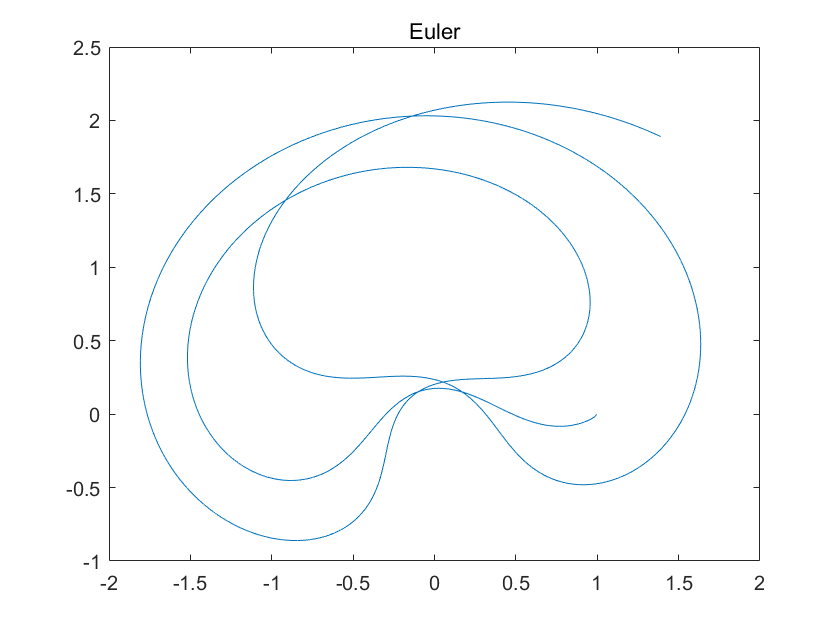
\includegraphics[scale=0.6]{../png/Euler.png}
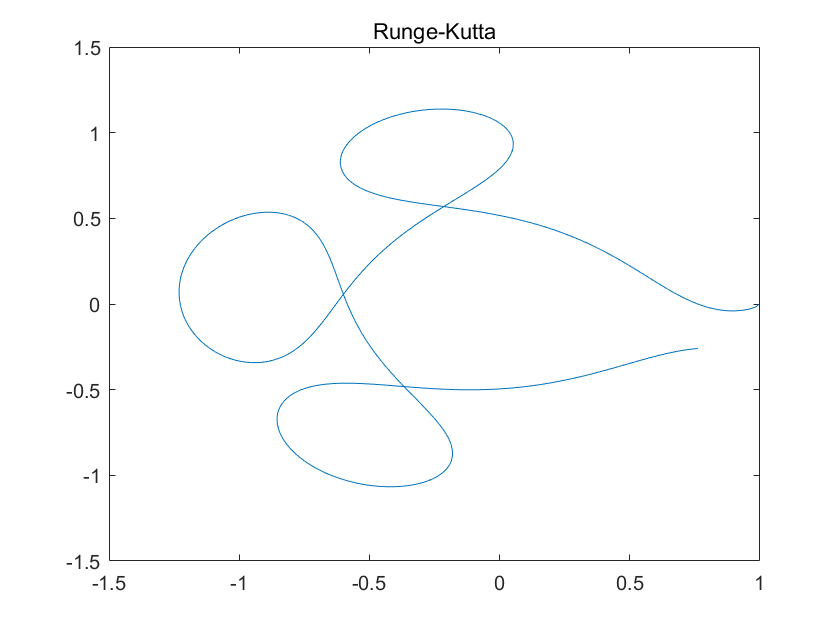
\includegraphics[scale=0.6]{../png/Runge-Kutta.png}

\raggedright
\hspace{0.8em}
从图中可以看到,Euler方法得到的图像是不稳定的,而Runge-Kutta方法得到的图像是稳定的,且已经比较接近精确解。具体的
原因从两种方法的稳定区域图可以看出,传统四阶Runge-Kutta方法的稳定区域更大,而Euler方法的稳定区域相对要小,所以导致了
Euler方法更容易不稳定。

\subsection*{IV-c. 对于第一个初值问题,不同方法达到误差$\mathbf{\leq10^{-3}}$所需要的CPU时间}
\hspace{0.8em}
下面结果中使用的是四阶Adams-Bashforth、五阶Adams-Moulton、四阶Bdfs以及传统的四阶Runge-Kutta
\\[12pt]
\centering
\renewcommand{\arraystretch}{2}
\begin{tabular}{|c|c|c|c|c|}
    \hline
            & \textbf{Adams}\ \textbf{Bashforth} & \textbf{Adams} \ \textbf{Moulton} & \textbf{Bdfs} & \textbf{Runge}\ \textbf{Kutta} \\
    \hline
    步数    & 390000                             & 90000                             & 370000        & 90000                          \\
    \hline
    误差    & 0.00100787                         & 0.000988293                       & 0.00105583    & 0.000988999                    \\
    \hline
    CPU时间 & 3.2193 s                           & 2.51664 s                         & 6.97739 s     & 2.24541 s                      \\
    \hline
\end{tabular}
\\[12pt]
\raggedright
从上表可以看出传统四阶Runge-Kutta方法表现最为优异。

\end{document}

%%% Local Variables: 
%%% mode: latex
%%% TeX-master: t
%%% End: 

